% Dandelion++ Propagation Diagram
% Shows stem phase (linear) transitioning to fluff phase (broadcast)
%
% ACCESSIBILITY ALT TEXT:
% A network diagram showing transaction propagation in two phases. Left
% (Stem Phase): A red origin node connects linearly through orange relay
% nodes S1, S2, S3 - hiding the true source. Right (Fluff Phase): After
% probabilistic transition, a green fluff source broadcasts to multiple
% blue nodes F1-F9 in a tree pattern. Legend explains that adversaries
% observing the fluff phase cannot determine the true origin, providing
% network-level privacy with plausible deniability.

\begin{figure}[ht]
\centering
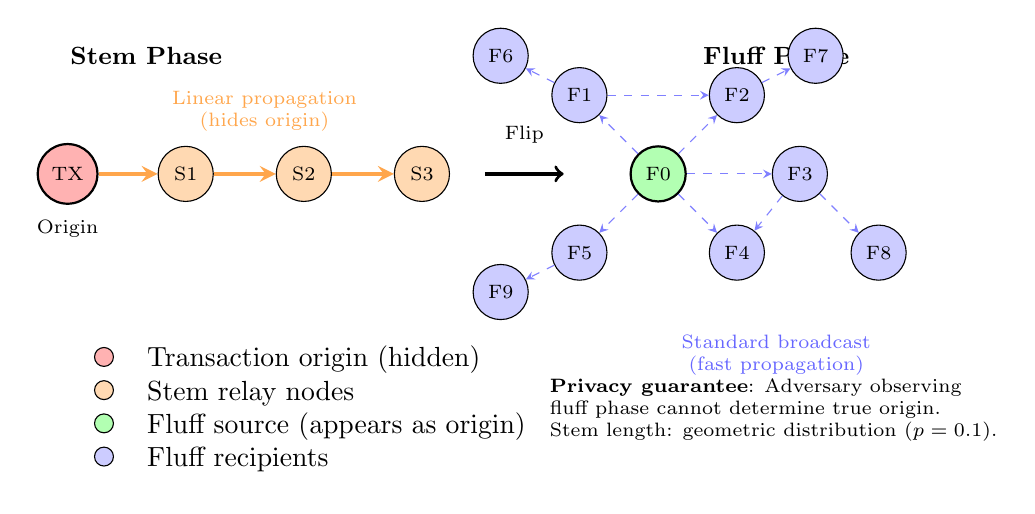
\begin{tikzpicture}[
    node distance=1.2cm,
    peer/.style={circle, draw, minimum size=0.7cm, font=\scriptsize},
    origin/.style={peer, fill=red!30, thick},
    stem/.style={peer, fill=orange!30},
    fluff/.style={peer, fill=blue!20},
    stempath/.style={->, >=stealth, thick, orange!70, line width=1.5pt},
    fluffpath/.style={->, >=stealth, dashed, blue!50},
    label/.style={font=\small\bfseries},
]

% === Stem Phase (left side) ===
\node[label] at (-4,3) {Stem Phase};

% Origin node
\node[origin] (o) at (-5,1.5) {TX};
\node[font=\scriptsize] at (-5,0.8) {Origin};

% Stem path nodes
\node[stem] (s1) at (-3.5,1.5) {S1};
\node[stem] (s2) at (-2,1.5) {S2};
\node[stem] (s3) at (-0.5,1.5) {S3};

% Stem arrows
\draw[stempath] (o) -- (s1);
\draw[stempath] (s1) -- (s2);
\draw[stempath] (s2) -- (s3);

% Stem annotation
\node[font=\scriptsize, align=center, orange!70] at (-2.5,2.3) {
    Linear propagation\\
    (hides origin)
};

% Transition marker
\draw[very thick, ->] (0.3,1.5) -- (1.3,1.5);
\node[font=\scriptsize] at (0.8,2) {Flip};

% === Fluff Phase (right side) ===
\node[label] at (4,3) {Fluff Phase};

% Fluff source (last stem node becomes fluff source)
\node[fluff, thick, fill=green!30] (f0) at (2.5,1.5) {F0};

% First ring of fluff nodes
\node[fluff] (f1) at (1.5,2.5) {F1};
\node[fluff] (f2) at (3.5,2.5) {F2};
\node[fluff] (f3) at (4.3,1.5) {F3};
\node[fluff] (f4) at (3.5,0.5) {F4};
\node[fluff] (f5) at (1.5,0.5) {F5};

% Second ring
\node[fluff] (f6) at (0.5,3) {F6};
\node[fluff] (f7) at (4.5,3) {F7};
\node[fluff] (f8) at (5.3,0.5) {F8};
\node[fluff] (f9) at (0.5,0) {F9};

% Fluff arrows from center
\draw[fluffpath] (f0) -- (f1);
\draw[fluffpath] (f0) -- (f2);
\draw[fluffpath] (f0) -- (f3);
\draw[fluffpath] (f0) -- (f4);
\draw[fluffpath] (f0) -- (f5);

% Fluff arrows from first ring
\draw[fluffpath] (f1) -- (f6);
\draw[fluffpath] (f2) -- (f7);
\draw[fluffpath] (f3) -- (f8);
\draw[fluffpath] (f5) -- (f9);

% Cross-connections in fluff
\draw[fluffpath] (f1) -- (f2);
\draw[fluffpath] (f3) -- (f4);

% Fluff annotation
\node[font=\scriptsize, align=center, blue!60] at (4,-0.8) {
    Standard broadcast\\
    (fast propagation)
};

% === Legend and explanation ===
\node[anchor=west] at (-5,-1.5) {
    \begin{tabular}{cl}
    \tikz\draw[fill=red!30, draw] (0,0) circle (0.12); & Transaction origin (hidden) \\
    \tikz\draw[fill=orange!30, draw] (0,0) circle (0.12); & Stem relay nodes \\
    \tikz\draw[fill=green!30, draw] (0,0) circle (0.12); & Fluff source (appears as origin) \\
    \tikz\draw[fill=blue!20, draw] (0,0) circle (0.12); & Fluff recipients \\
    \end{tabular}
};

% Privacy note
\node[align=left, font=\scriptsize, anchor=west] at (1,-1.5) {
    \textbf{Privacy guarantee}: Adversary observing\\
    fluff phase cannot determine true origin.\\
    Stem length: geometric distribution ($p = 0.1$).
};

\end{tikzpicture}
\caption{Dandelion++ transaction propagation~\cite{dandelion}. In the \textit{stem phase},
transactions propagate along a random linear path, obscuring the origin. After
a probabilistic transition (average 10 hops), the \textit{fluff phase} begins:
standard broadcast propagation for fast network-wide dissemination. The fluff
source appears to be the transaction origin, providing plausible deniability
for the true sender.}
\label{fig:dandelion}
\end{figure}
